\section{Numerical Results}
\label{sec:numerical_results}
To verify the performance of the proposed method we test it on two different 3D problems: a cantilever beam and the Stanford bunny. Both geometries use material properties designed to mimic soft tissue behavior, with Young's modulus $E = 10^6$ Pa and Poisson's ratio $\nu = 0.45$.

\subsubsection*{Cantilever beam}
\label{sec:cantilever_beam_setup}
The first test case is a cantilever beam with a square cross-section of size $1 \times 1$ and a length of $10$. The beam is clamped at one end and free at the other. This geometry represents a classical benchmark problem in structural mechanics, allowing for clear interpretation of the modal behavior and providing a controlled environment to validate the fundamental capabilities of our neural network approach. The cantilever beam exhibits well-understood physics with distinct modal patterns: bending modes in two perpendicular directions, torsional modes, and higher-order coupled deformation modes. The soft tissue material properties result in large deformations under relatively small loads, making this an ideal test case for nonlinear mechanics validation.

\subsubsection*{Stanford bunny}
\label{sec:stanford_bunny_setup}
The second test case employs the Stanford bunny \cite{bunny-mesh}, a widely recognized benchmark geometry in computational mechanics and computer graphics. This complex 3D shape presents a significantly more challenging validation scenario due to its intricate surface topology, non-uniform geometry, and irregular mass distribution. The Stanford bunny is fixed at its base and subjected to various loading conditions to generate the training data for the POD-based model reduction. This geometry tests the robustness and generalization capabilities of our method on realistic, non-trivial shapes that are commonly encountered in biomedical engineering applications. The complex geometry introduces coupling between different deformation modes and provides a stringent test for the neural network's ability to capture intricate displacement patterns typical of soft biological tissues.

\begin{figure}[H]
    \centering
    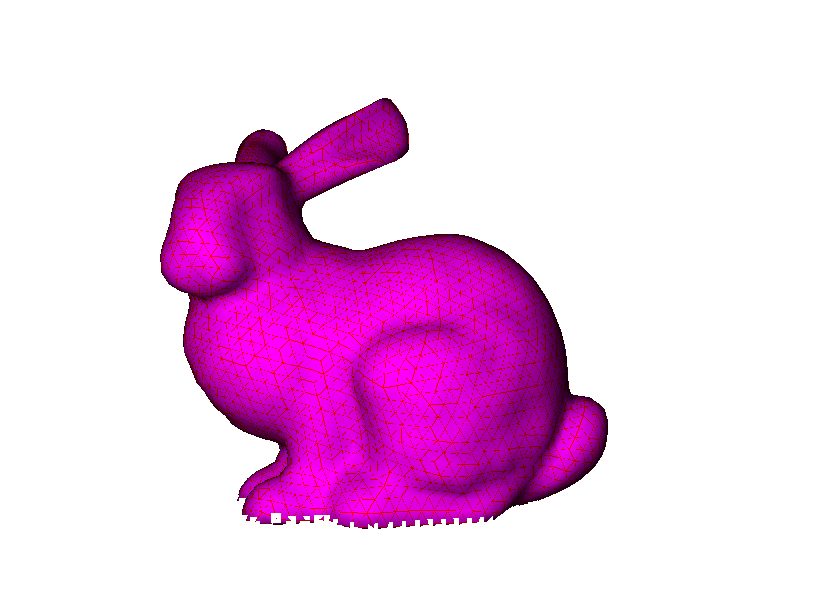
\includegraphics[width=0.7\textwidth]{Images/stanford_bunny.png}
    \caption{The Stanford bunny geometry used in the tests.}
    \label{fig:stanford_bunny}
    \end{figure}

Both geometries are discretized using tetrahedral finite elements, with mesh refinement studies performed to ensure convergence of the full-order solutions. The cantilever beam uses approximately 800 elements, while the Stanford bunny requires around 22000 elements.
\subsection{Optimal number of modes}
\label{sec:optimal_number_modes}
One of the first steps is clearly to determine the optimal number of modes to be used in the approximation. If we choose too few modes, the approximation will not be accurate enough, but choosing too many modes only increases the complexity of the reduced model, with diminishing returns in terms of accuracy. The figure \ref{fig:optimal_number_modes} shows the error in the approximation of the displacement field as a function of the number of modes used. The error is computed as the Root Mean Square Error (RMSE) between the displacement field computed with the full model and the one computed with the reduced model. The RMSE is defined as:
\begin{equation}
    RMSE = \sqrt{\frac{1}{N}\sum_{i=1}^N (\bm{u}_i^{full} - \bm{u}_i^{reduced})^2},
\end{equation}
where $N$ is the number of nodes in the mesh, $\bm{u}_i^{full}$ is the displacement field computed with the full model and $\bm{u}_i^{reduced}$ is the displacement field computed with the reduced model. The figure shows that the error decreases rapidly with the number of modes used, and then stabilizes around 20 modes. We can see that with 10 modes the error is already below \(10^{-3}\) and with 20 modes the error is below \(10^{-4}\). For our use case, 7 modes are sufficient.
\begin{figure}[H]
    \centering
    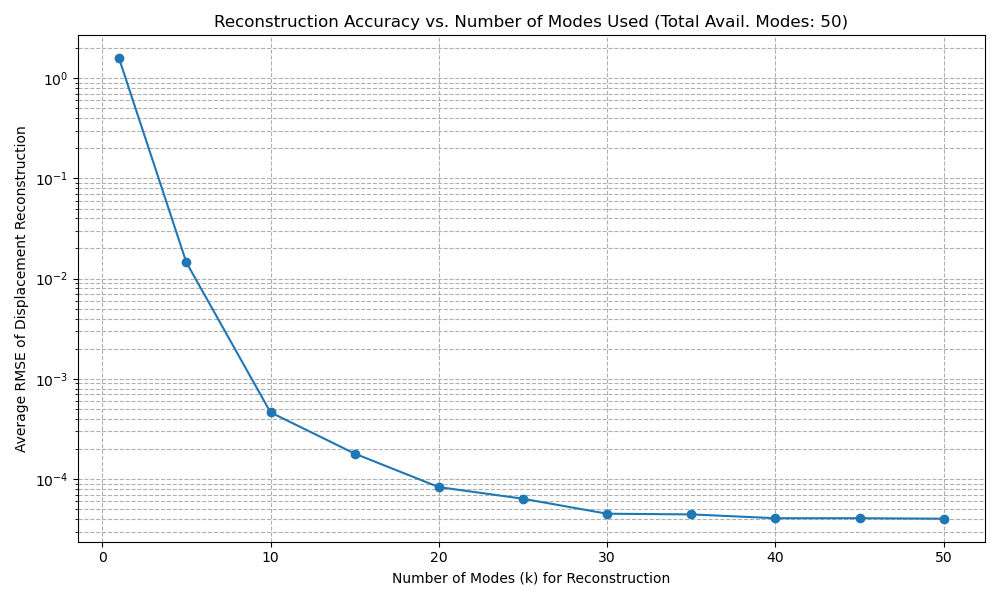
\includegraphics[width=0.7\textwidth]{Images/rmse_vs_modes.png}
    \caption{RMSE of the displacement field as a function of the number of modes used.}
    \label{fig:optimal_number_modes}
\end{figure}

\subsection{Training the model}
\label{sec:training_model}
The next step is to train the model using a supervised learning approach. For this purpose, we generate comprehensive datasets of labeled training examples for both geometries. The training data consists of pairs $(z, u, E)$ where $z$ represents the modal coordinates vector, $u$ is the corresponding displacement field, and $E$ is the associated mechanical energy of the deformed configuration.
For the cantilever beam, we create a dataset of 600 deformations by applying different combinations of modal forces to the structure while maintaining the fixed boundary condition at one end. 

For each combination of modal forces, we solve the static equilibrium problem using the full-order FEM solver to obtain the corresponding displacement field and mechanical energy. The resulting displacement field is then projected onto the modal basis to extract the modal coordinates $z$, forming training pairs $(z, u, E)$.

For the Stanford bunny geometry, we generate a dataset of 500 deformations using a similar sampling strategy. The modal coefficient ranges are determined based on preliminary analysis of the bunny's natural vibration modes and their relative contribution to physically realistic deformations.

Each training sample is generated by first selecting a random combination of modal coordinates within the specified ranges, then computing the corresponding displacement field and total mechanical energy using the full-order FEM solver. This supervised approach ensures that the neural network learns from accurate, physics-based ground truth data.

The neural network is trained to simultaneously predict both the displacement field and the mechanical energy given the modal coordinates as input. This multi-output formulation allows the model to learn the coupled relationship between geometric deformation and energy, which is crucial for maintaining physical consistency during predictions. The network architecture consists of fully connected layers with appropriate activation functions to capture the nonlinear mapping from modal space to the physical displacement and energy fields.

The training process is described in detail in Section \ref{sec:training_neural_modes}.

For the cantilever beam, we stopped the training, after 200 epochs, when the loss reached a plateau and we observed no significant improvement in the last 50 epochs. In Figure \ref{fig:training_loss_beam} we can see the training loss for the cantilever beam, which shows that immediately after the first epoch the loss drops significantly, meaning that the model is able to learn the underlying physics of the problem very quickly. We then let the model train for 200 so that it can receive as input a wide range of different configurations and be able to generalize well.

\begin{figure}[H]
    \centering
    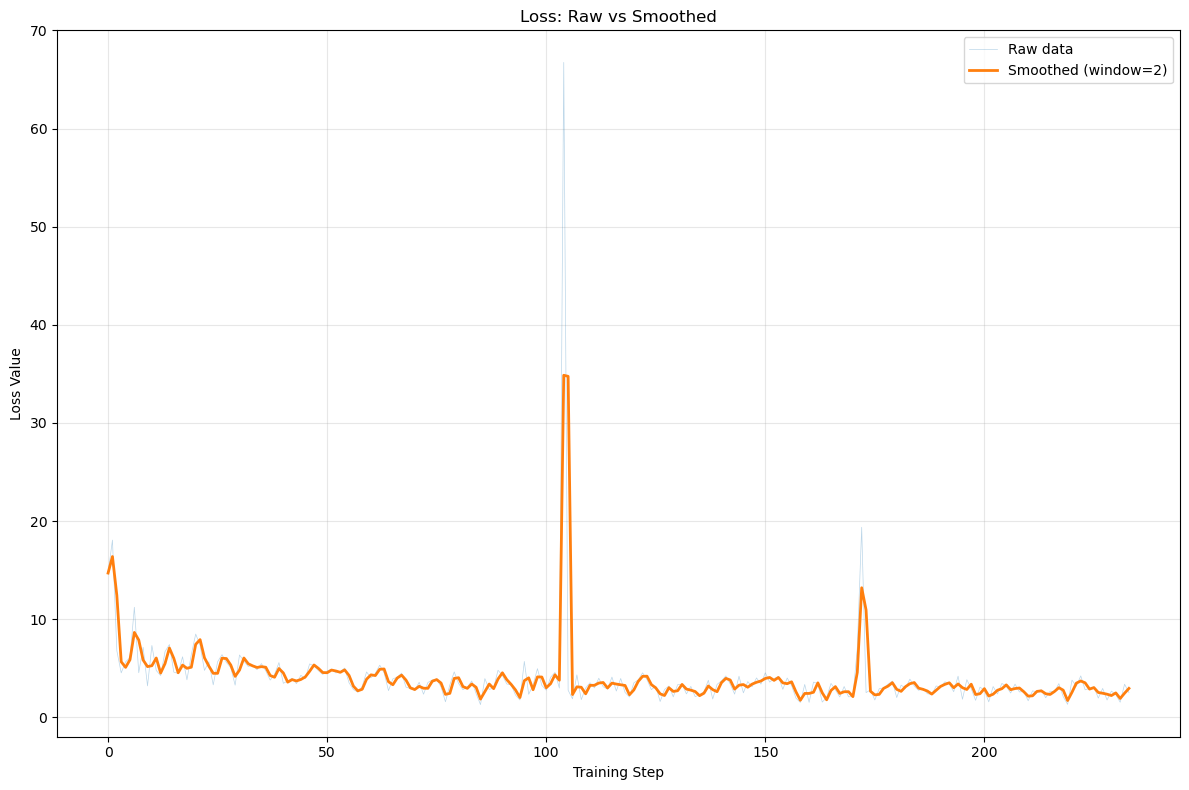
\includegraphics[width=0.7\textwidth]{Images/training_loss_smoothed.png}
    \caption{Training loss for the cantilever beam.}
    \label{fig:training_loss_beam}
\end{figure}

We also provide the plot of the energy part of the loss function, which is computed as the mean of the internal energy of the batch of training samples. As we can see in Figure \ref{fig:training_energy_loss_beam}, at the first epoch the energy is very high, because the last layer of the neural network is set to have zero weights and biases, meaning that at the end of first epoch the prediction is just the linear modes approximation, then the energy loss drops significantly in the first few epochs, learning a meaningful correction to the linear modes approximation, while maintaning the ability to generalize even though the training set is not very large. The energy loss stabilizes around \(5e3\), which is on par with the energy computed in the validation phase with the full-order FEM solver.

\begin{figure}[H]
    \centering
    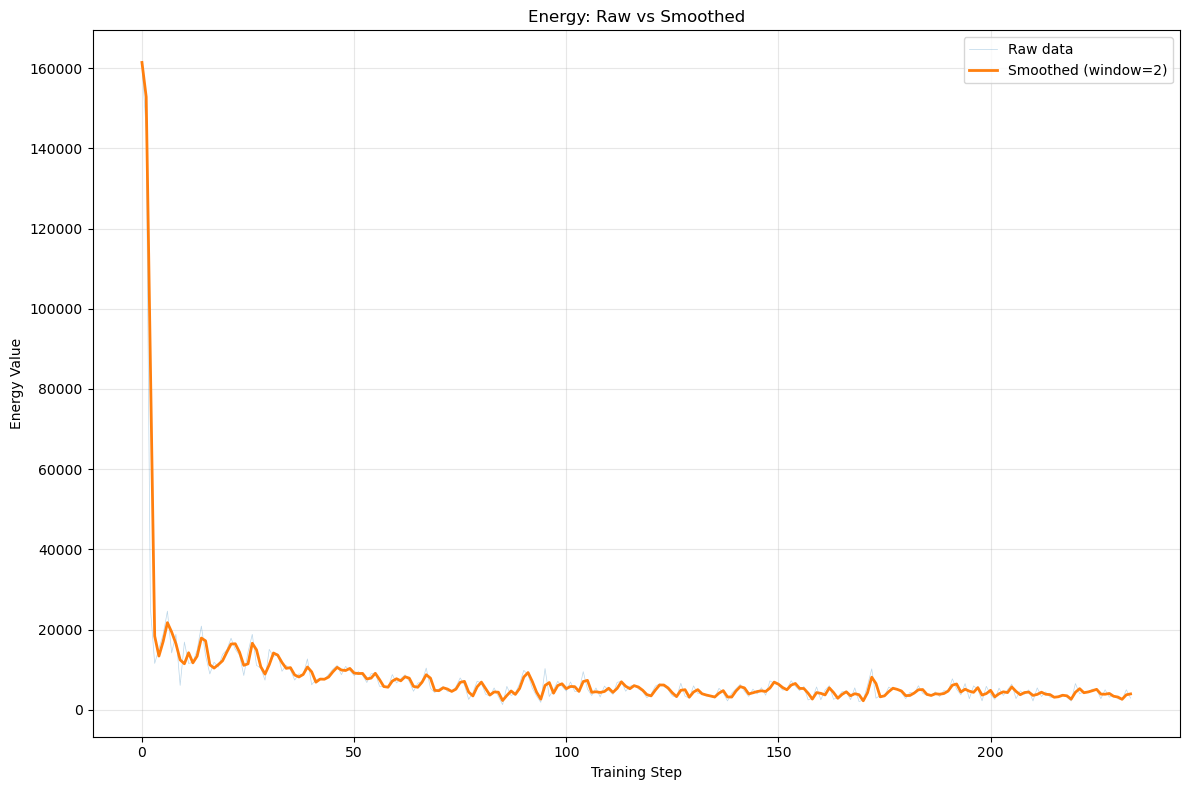
\includegraphics[width=0.7\textwidth]{Images/training_energy_smoothed.png}
    \caption{Training energy loss for the cantilever beam.}
    \label{fig:training_energy_loss_beam}
\end{figure}


\subsection{Testing the model}
\label{sec:testing_model}
Since the training is completely data-free we perform the validation of the model in two main ways. The first one is to check the accuracy of reconstruction of the displacement field for some random static configurations, given by applying random coefficients to the modal forces. The second way of validation is to see how well the model can predict the displacement field for a dynamic problem, where the FEM solver is used to compute the first two time steps of the dynamic problem, and then the equation \ref{eq:optimization_problem} is used to predict the next time steps. 

\subsubsection{Self-supervised training}
\label{sec:self_supervised_training}
To provide some insight into the self-supervised training process, we trained a network following the procedure described by \cite{Wang_Du_Coros_Thomaszewski_2024}, where the network is trained by using only the minimization of the energy loss function, without any ground truth data. The training is performed by sampling uniformly the modal coefficients within the ranges established during the training phase:
\begin{align*}
    z_1 &\in [-225, 225], \\
    z_2 &\in [-170, 170], \\
    z_3 &\in [-20, 20], \\
    z_4 &\in [-15, 15], \\
    z_5 &\in [-5, 5], \\
    z_6 &\in [-80, 80], \\
    z_7 &\in [-170, 170].
\end{align*}

Then we perform the validation of the model on the same validation set used for the supervised training. The result are shown in Figure \ref{fig:self_supervised_validation_mse_comparison}, where we can see that the self-supervised model performs at most as well as the linear modes model, which means that it is not worth to use such a model, since it does not provide any significant advantage over the linear modes. 

\begin{figure}[H]
    \centering
    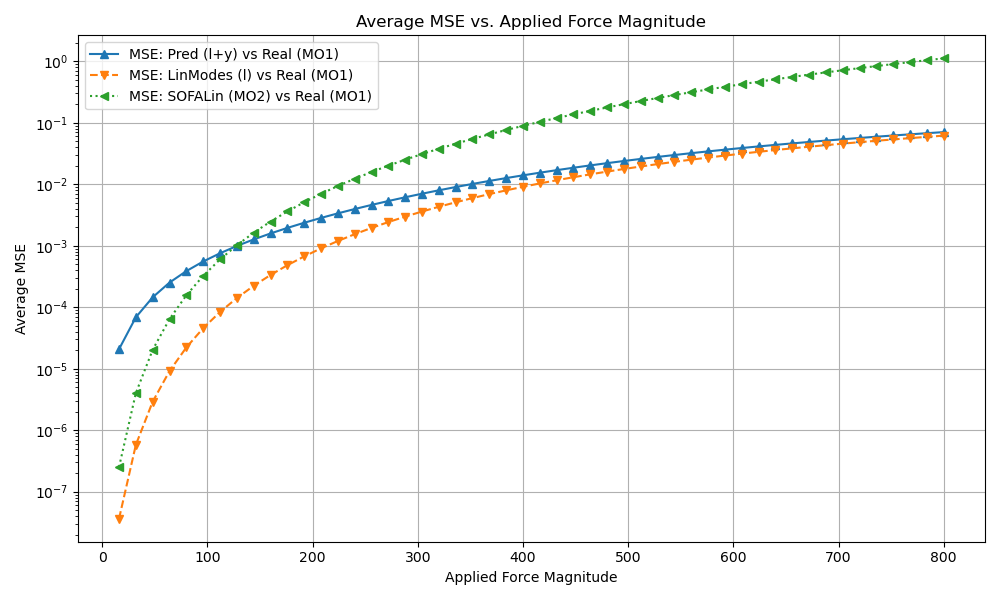
\includegraphics[width=0.8\textwidth]{Images/self_supervised_mse.png}
    \caption{Average MSE between 40 different simulations with randomly applied forces. The neural modes model (blue) is compared against the linear modes model (orange) and the linear FEM model (green), all evaluated against the nonlinear FEM ground truth. The self-supervised model performs at most as well as the linear modes, as shown by the MSE values.}
    \label{fig:self_supervised_validation_mse_comparison}
\end{figure}

\subsubsection{Static validation}
\label{sec:static_validation}
For the static validation phase, we rigorously test the neural network model's ability to accurately reconstruct displacement fields for various static configurations that were not seen during training. This validation is crucial to establish confidence in the model's interpolation capabilities within the trained parameter space and to verify that the network has successfully learned the underlying physics of the structural mechanics problem.


We generate a comprehensive test dataset consisting of 100 random static configurations by sampling modal coefficients uniformly within the established training ranges for each mode. Each test case represents a unique static equilibrium state of the cantilever beam under different loading conditions. For each configuration, we compute the reference displacement field using the full-order FEM solver and compare it with the neural network's prediction. The comparison is performed both qualitatively through visual inspection of the displacement fields and quantitatively using the Root Mean Square Error (RMSE) metric.

At 800N of applied force, the maximum MSE is $10^{-3}$ for the neural model, significantly outperforming both the linear modes model ($10^{-3}$) and the FEM with linear elasticity ($10^{-2}$). The maximum observed error across all test cases is $1.2 \times 10^{-3}$, while the minimum is $1.2 \times 10^{-5}$, demonstrating that the model maintains excellent accuracy across the entire range of test configurations. Importantly, the neural network error remains bounded within this narrow range ($10^{-5}$ to $10^{-3}$) across all force magnitudes, making it significantly more reliable than linear modes, which perform very well for small displacements but exhibit exponentially growing errors when operating outside the small deformation range. These results confirm that the neural network has successfully learned to approximate the complex nonlinear relationship between modal coordinates and the resulting displacement fields with remarkable precision and consistent reliability.

Figure \ref{fig:static_mse_comparison} presents the average MSE comparison between three different approaches: neural modes, linear modes, and linear FEM, all evaluated against the nonlinear FEM ground truth across force magnitudes ranging from 0 to 800 N. The results reveal distinct performance characteristics across different deformation regimes. For small displacements in the linear range (low forces), the linear modes approach demonstrates superior accuracy due to its exact representation of the underlying linear physics. However, as the applied forces increase and the system enters the nonlinear deformation regime, the neural modes approach significantly outperforms both linear methods by approximately an order of magnitude. This performance crossover occurs around 100 N, where the geometric nonlinearities become dominant. The superior performance of neural modes in the nonlinear range validates the method's ability to capture complex deformation patterns that cannot be represented by linear modal decomposition alone.

\begin{figure}[H]
    \centering
    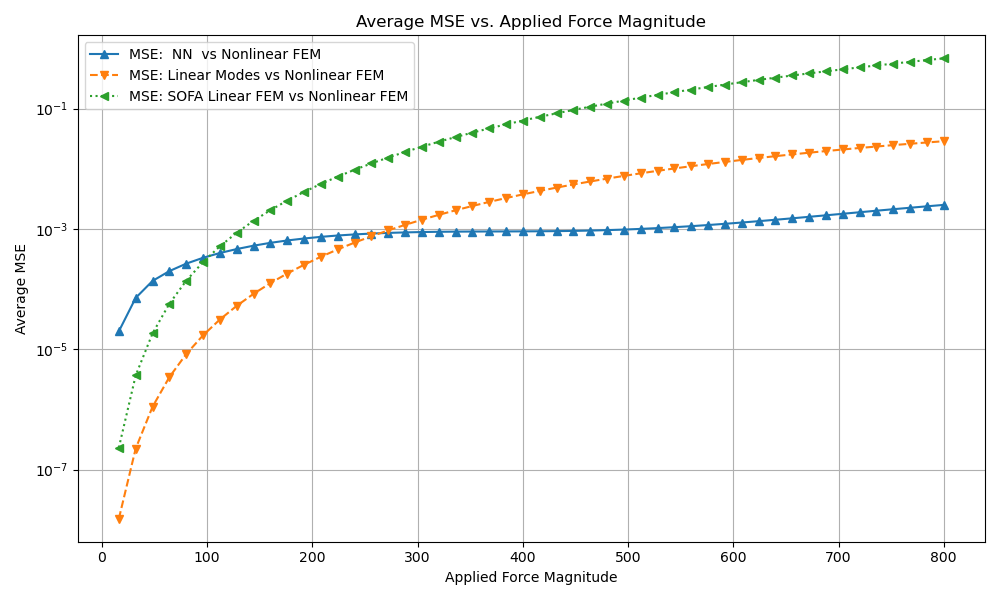
\includegraphics[width=0.8\textwidth]{Images/beam_static_mse.png}
    \caption{Average MSE between 40 different simulations with randomly applied forces. The neural modes model (blue) is compared against the linear modes model (orange) and the linear FEM model (green), all evaluated against the nonlinear FEM ground truth. The neural modes model significantly outperforms the linear modes, especially in the nonlinear regime.}
    \label{fig:static_mse_comparison}
\end{figure}

To provide an additional layer of insight into the model's performance, Figure \ref{fig:static_energy_beam} illustrates the relationship between the applied force and the internal mechanical energy of the beam. The graph compares the energy computed by the neural network model against the ground truth obtained from the nonlinear FEM solution. As we can see again, in the small deformation regime, the linear modes outperform the neural modes, keeping the internal energy closer  to the ground truth. However, as the applied force increases and the beam undergoes larger deformations, the neural modes model manages to correct the linear model into a lower energy state, which is closer to the ground truth even in the case of large deformations. 
\begin{figure}[H]
    \centering
    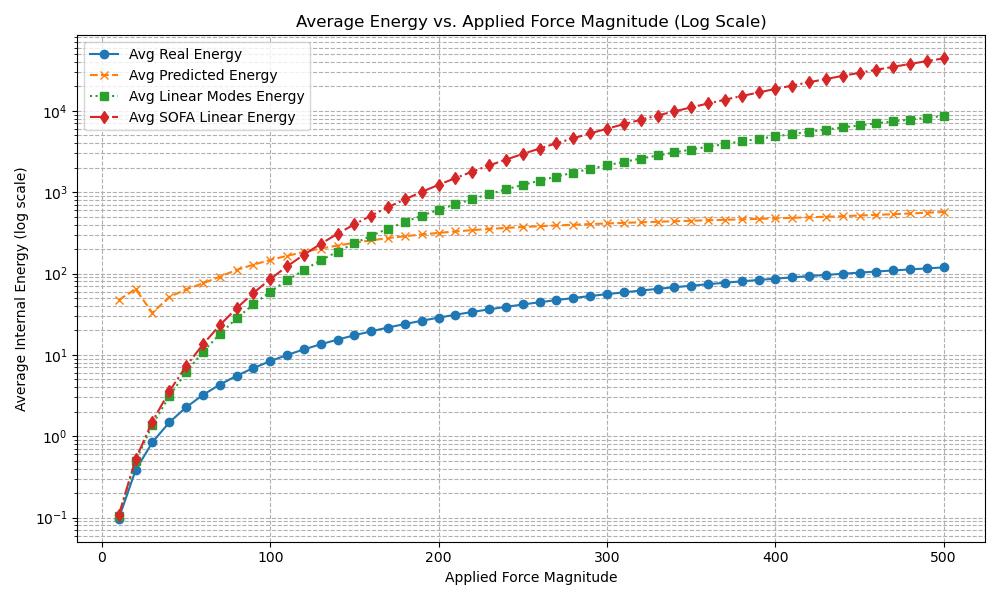
\includegraphics[width=0.8\textwidth]{Images/beam_static_energy.png}
    \caption{Internal mechanical energy of the beam as a function of the applied force. The orange line represents the energy computed by the neural network model, while the blue line is the ground truth obtained from the nonlinear FEM solution. The red line represents the energy computed by the FEM with linear elasticity and the green line is the energy computed by the linear modes model.}
    \label{fig:static_energy_beam}
\end{figure}


Figure \ref{fig:static_rmse_distribution} provides a detailed visual comparison of the different modeling approaches applied to a representative beam deformation case. In this visualization, we can observe the predicted deformation patterns from four different computational methods: the neural network prediction (shown in magenta), the ground truth nonlinear FEM solution (displayed in green), the linear modes approximation (represented by the red wireframe), and the linear FEM model (illustrated by the blue wireframe). 

This particular example demonstrates a critical limitation of linear approaches when dealing with large deformations. The linear modes and linear FEM models tend to significantly underestimate the pronounced bending curvature that develops in the beam under substantial loading conditions. This loss of geometric fidelity represents a fundamental limitation of linear modeling approaches, as they cannot adequately capture the inherent nonlinear geometric effects that become dominant in large-deformation scenarios. The accentuated bending behavior observed in the ground truth solution is a characteristic manifestation of geometric nonlinearity, where the deformed configuration significantly influences the structural response.

On the other hand, the neural modes approach successfully captures this complex nonlinear deformation pattern with remarkable accuracy. The magenta neural network prediction closely follows the green ground truth solution, demonstrating the model's capability to learn and reproduce the intricate relationships between modal coordinates and the resulting nonlinear displacement fields. This superior performance in capturing geometric nonlinearities represents one of the key advantages of the proposed neural modes' methodology over traditional linear model reduction techniques, particularly for applications involving soft tissues and other materials that undergo large deformations during normal operation.

\begin{figure}[H]
    \centering
    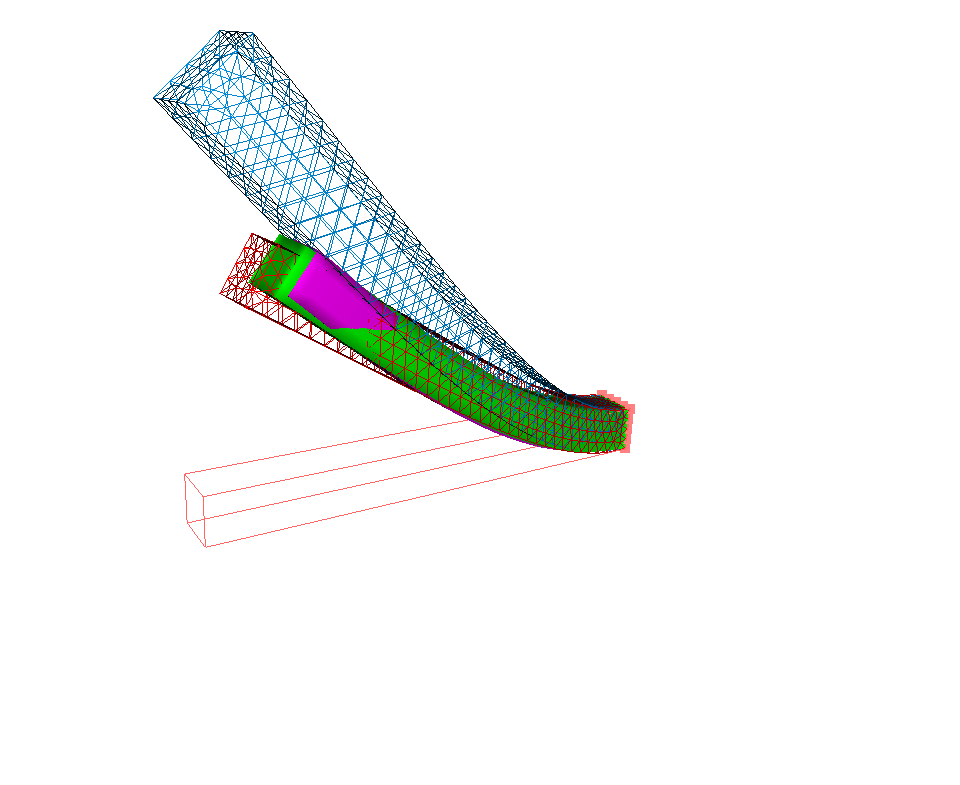
\includegraphics[width=0.4\textwidth]{Images/sofa_example_beam.png}
    \caption{Example of a static reconstruction in the case of the beam. The magenta beam represents the neural network prediction, the green one is the ground truth, the red wireframe represents the linear modes and the blue wireframe is the linear FEM model.}
    \label{fig:static_rmse_distribution}
\end{figure}

In the case of the Stanford bunny, the static validation follows a similar procedure. We generate a test dataset of 50 random configurations by sampling modal coefficients uniformly within the ranges established during training. Each configuration is then processed through the neural network to obtain the predicted displacement field, and grouped by the corresponding force applied to the bunny. The neural network's predictions are compared against the reference displacement fields computed using the full-order FEM solver equipped with the Neo-Hookean hyperelastic model, the linear modes approximation, and the linear FEM model.

Figure \ref{fig:static_mse_bunny} presents the average MSE comparison between the neural modes, linear modes, and linear FEM approaches across different force magnitudes applied to the Stanford bunny. The results reveal a similar trend to that observed in the cantilever beam case. For small forces, the linear modes approach performs well, but as the applied force increases and the bunny undergoes larger deformations, the neural modes model significantly outperforms both linear methods. The neural network achieves an order of magnitude improvement in accuracy compared to linear modes, demonstrating its ability to capture complex nonlinear deformation patterns that are not adequately represented by linear modal decomposition.
\begin{figure}[H]
    \centering
    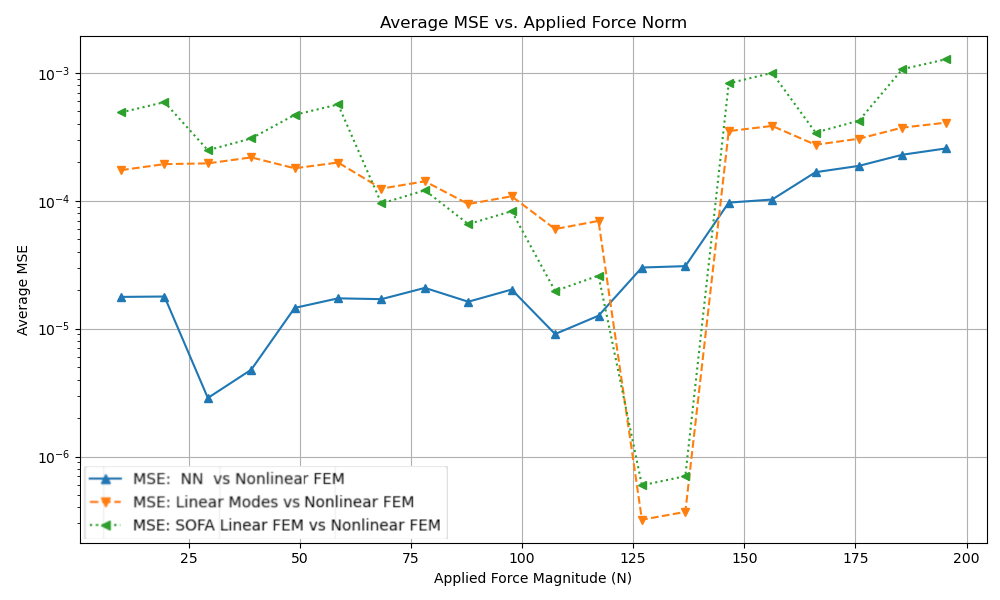
\includegraphics[width=0.8\textwidth]{Images/bunny_static_mse.png}
    \caption{Average MSE between 50 different simulations with randomly applied forces on the Stanford bunny.}
    \label{fig:static_mse_bunny}
    \end{figure}

Also in this case, Figure \ref{fig:static_energy_bunny} illustrates the relationship between the applied force and the internal mechanical energy of the object. Again, we have energies that are lower by an order of magnitude than the linear modes and two orders of magnitude lower than the linear FEM model. In the case of the bunny the energy datum is particularly important, as the principal modes of deformation of the object are related to his head and ears, which means that most of its body is not deformed, keeping the MSE between the predicted displacement field and the ground truth very low, even if the prediction is far from being correct. Having that many nodes that stay still even in the deformed configuration, calls for additional metrics to evaluate the performance of the model, such as the internal energy, which we observe has a tendency to explode using linear elasticity or a combination of linear modes, but in the case of the neural modes model, the energy is just a bit higher than the ground truth.

\begin{figure}[H]
    \centering
    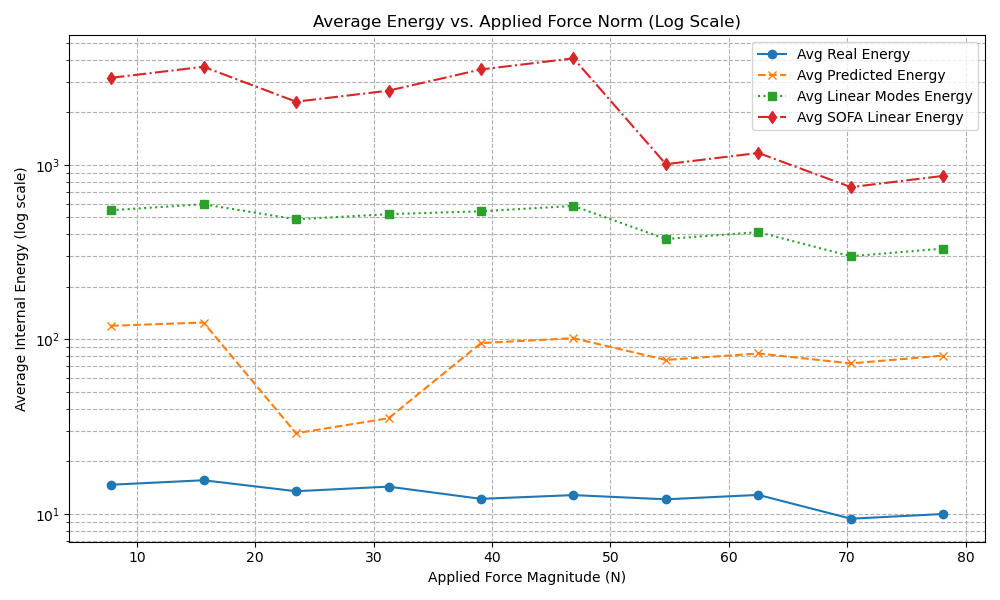
\includegraphics[width=0.8\textwidth]{Images/bunny_static_energy.png}
    \caption{Internal mechanical energy of the Stanford bunny as a function of the applied force. The orange line represents the energy computed by the neural network model, while the blue line is the ground truth obtained from the nonlinear FEM solution. The red line represents the energy computed by the FEM with linear elasticity and the green line is the energy computed by the linear modes model.}
    \label{fig:static_energy_bunny}
    \end{figure}
In  Figure \ref{fig:sofa_example_bunny} we can see an example of a static reconstruction in the case of the Stanford bunny. The magenta bunny represents the neural network prediction, the green one is the ground truth, the red wireframe represents the linear modes and the blue wireframe is the linear FEM model. As we can see, the force is applied  to the ears of the bunny, which are the most deformable parts of the geometry and exhibit a highly nonlinear behavior, as confirmed by the significant differences between the Neo-Hookean ground truth and the linear elasticity FEM model. The neural network prediction closely follows the ground truth, while the linear modes tends to amplify the volume of the ears and fail to reconstruct the bending behavior of them.

\begin{figure}[H]
    \centering
    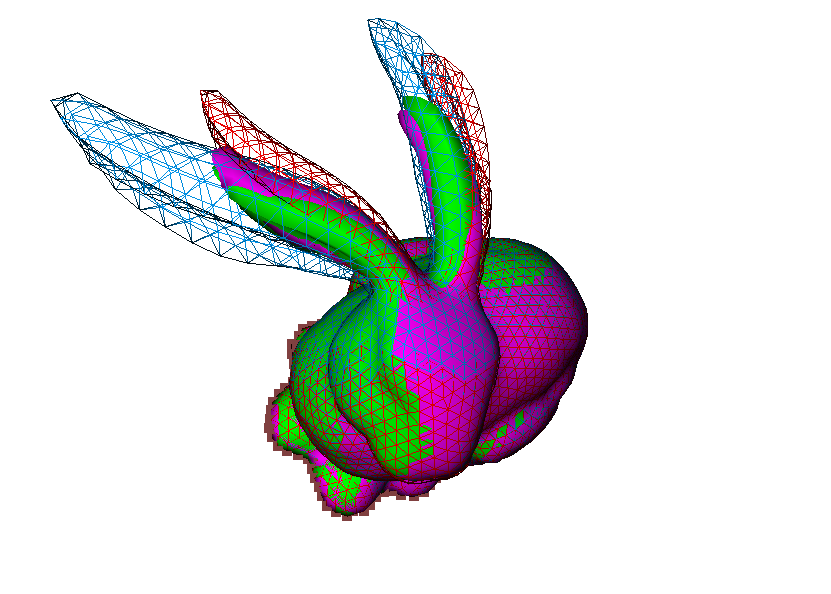
\includegraphics[width=0.4\textwidth]{Images/sofa_example_bunny.png}
    \caption{Example of a static reconstruction in the case of the Stanford bunny. The magenta bunny represents the neural network prediction, the green one is the ground truth, the red wireframe represents the linear modes and the blue wireframe is the linear FEM model.}
    \label{fig:sofa_example_bunny}
    \end{figure}
    
\subsubsection{Interpretability}
Another important aspect of this framework is its interpretability. While neural networks have a tendency to be completely black boxes, meaning that it is very hard to understand how a small change in the input can lead to a change in the output, in this case, the model is easily interpretable, since the input is a vector of coefficients that are then used to compute the displacement field using the modal basis. While linear modes are computed just as 
\begin{equation*}
    \bm{u} = \sum_{i=1}^n z_i \bm{\phi}_i,
    \end{equation*}
    the neural modes model computes the displacement field as
    \begin{equation*}
    \bm{u} = \sum_{i=1}^n z_i \bm{\phi}_i + \bm{f}(z),
    \end{equation*}
    where $\bm{f}(z)$ is the output of the neural network. This means that using a vector that has zero coefficients in all, but one of the modes, we can easily see how the neural network modifies the displacement field in that particular mode. This is a very important feature, since it allows us to understand how the neural network is modifying the displacement field in each mode, and how it is able to capture the nonlinear behavior of the system. 
    In Figure \ref{fig:latent_space_viz} we can see a visualization of the latent space of the neural modes model for the Stanford bunny and the 7 corresponding modes. We see that coefficients for the vector tend to decrease as we move from the first mode to the last one, which is on par with what we experienced when we faced the question of the optimal sampling of the latent space in Section \ref{sec:sampling_modal_space}.

\begin{figure}[H]
    \centering
    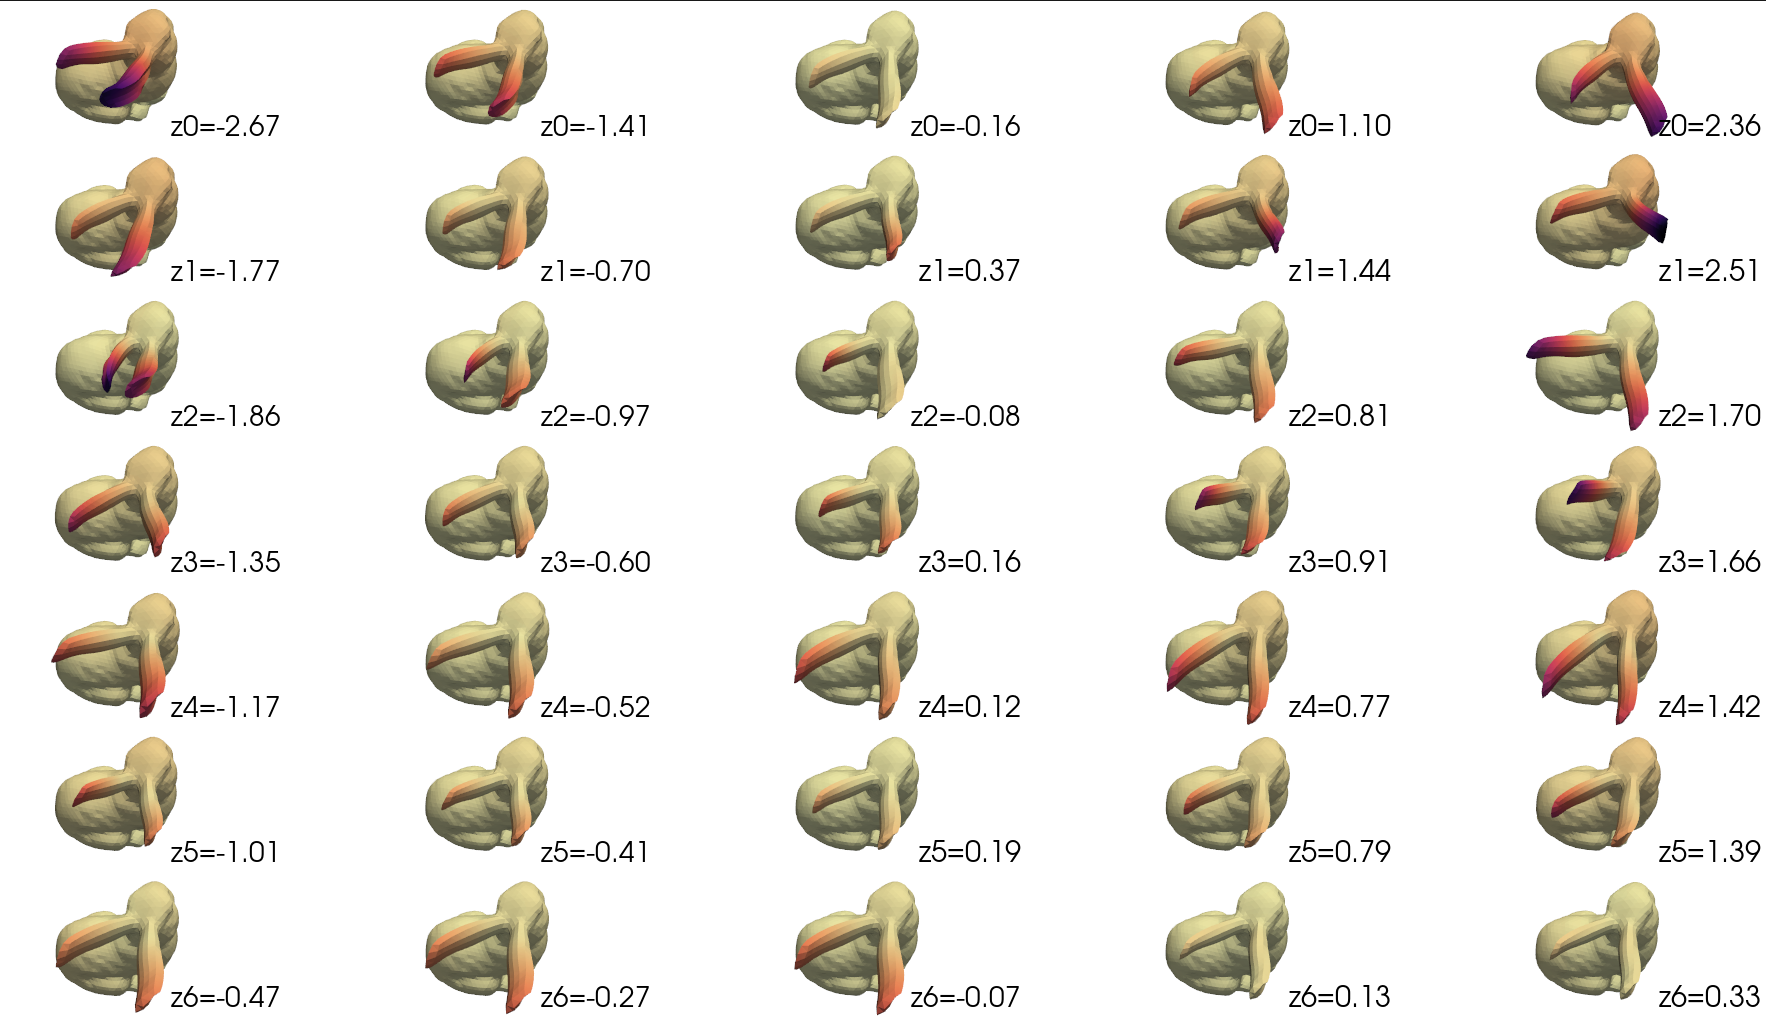
\includegraphics[width=\textwidth]{Images/latent_space_viz.png}
    \caption{Visualization of the latent space of the neural modes model for the Stanford bunny. Each row represents a different mode, and in the corner we can se the actual value of the coefficient for that mode. The first column represents the most significant mode, which describes the overall movement of the head of the bunny.}
    \label{fig:latent_space_viz}
    \end{figure}
    

\subsubsection{Dynamic validation}
\label{sec:dynamic_validation}
The dynamic validation represents a more challenging and comprehensive test of the neural network model's capabilities, as it evaluates the model's performance in predicting time-dependent structural behavior over extended simulation periods. Unlike static validation, dynamic problems involve the accumulation of errors ove200r time, making this validation particularly stringent and representative of real-world applications where the model would be used for long-term predictions.

For the dynamic validation procedure, we implement a hybrid approach where the first two time steps are computed using the full-order FEM solver to establish accurate initial conditions, including both displacement and velocity fields. Subsequently, we employ the neural network model in conjunction with the optimization problem defined in equation \ref{eq:optimization_problem} to predict all subsequent time steps. This methodology allows us to assess how well the model can maintain physical consistency and accuracy when operating in a predictive mode over extended time horizons.

In reality, just performing the first two time steps with the FEM solver is definitely not enough to obtain two time steps that are representative of the dynamic behavior of the system, so, our testing environment is set up to run the first 100 time steps with the FEM solver, and then take the last two time steps to initialize the neural network model. Then we let it run until we see a significant divergence from the ground truth, which happens after around 120 steps. While this results seems less than ideal, it paves the way for future work to improve the underlying model and also fine tune the optimization problem to obtain a more accurate prediction.

As we can see from the  results, the neural network model performance in terms of MSE is just slightly better than the linear modes model, which raises questions about the need of  using a neural network for this problem. This is a perfectly valid concern, since the linear modes model is already a very good approximation of the displacement field, and it is much simpler to implement. As we can see in Figure \ref{fig:dynamic_validation_mse_comparison}, both the neural modes and linear modes models stray further from the ground truth as time progresses, but the neural modes model does slightly better, especially in the initial steps. When we reach the last part of the simulation, the MSE of the neural modes model is around 0.1, which clearly means that the prediction is not very accurate.

\begin{figure}[H]
    \centering
    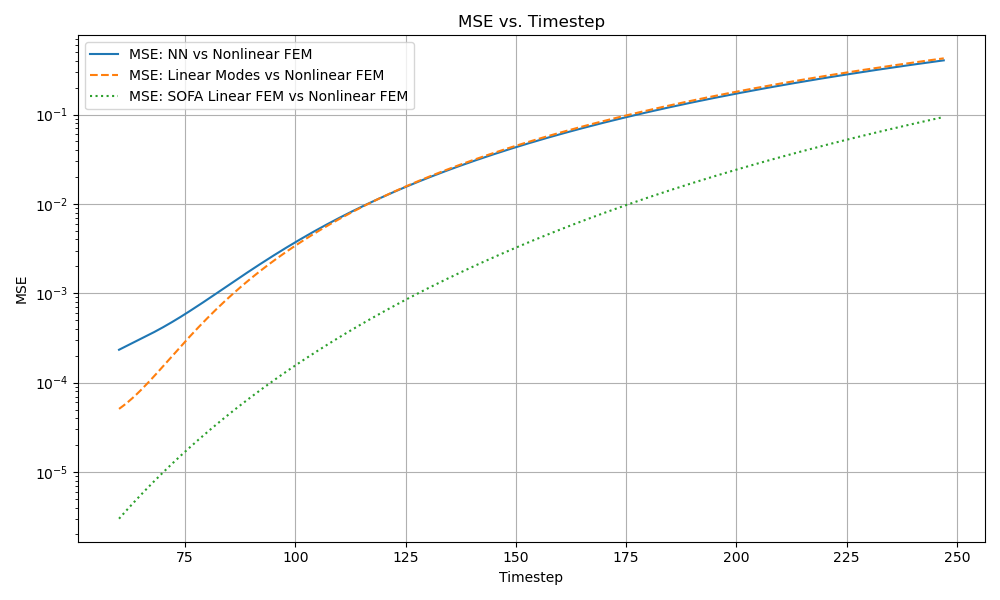
\includegraphics[width=0.8\textwidth]{Images/beam_dynamic_mse.png}
    \caption{MSE of the displacement field as a function of time for the dynamic validation of the cantilever beam. The neural modes model (blue) and the linear modes model (orange) are compared against the ground truth obtained from the nonlinear FEM solution (green). The neural modes model performs slightly better than the linear modes model, especially after the first few time steps.}
    \label{fig:dynamic_validation_mse_comparison}
    \end{figure}

Things change drastically when we take a look at the internal energy of the system, as we can see in Figure \ref{fig:dynamic_validation_energy_comparison}. The neural modes model manages to keep the energy at a level that is much closer to the ground truth, while the linear modes model diverges significantly from it. This means that, while both models are not very accurate in terms of displacement field, the neural modes model is able to obtain physically plausible and realistic predictions, which is still a good result, comparing to the other dynamic models we have seen in the literature, considering that the neural modes model is trained only on static data, and does not use any dynamic information to learn the underlying physics of the system, and that lowers the computational cost of the training phase significantly. The linear modes model, on the other hand, diverges from the ground truth in terms of energy, which is a classic limitation of linear models when dealing with large deformations. Outside the linear regime, linear models tend to ``explode'' in terms of energy and volume, due to the inherent shortcomings of linear elasticity in capturing the complex behavior of materials.

\begin{figure}[htb]
    \centering
    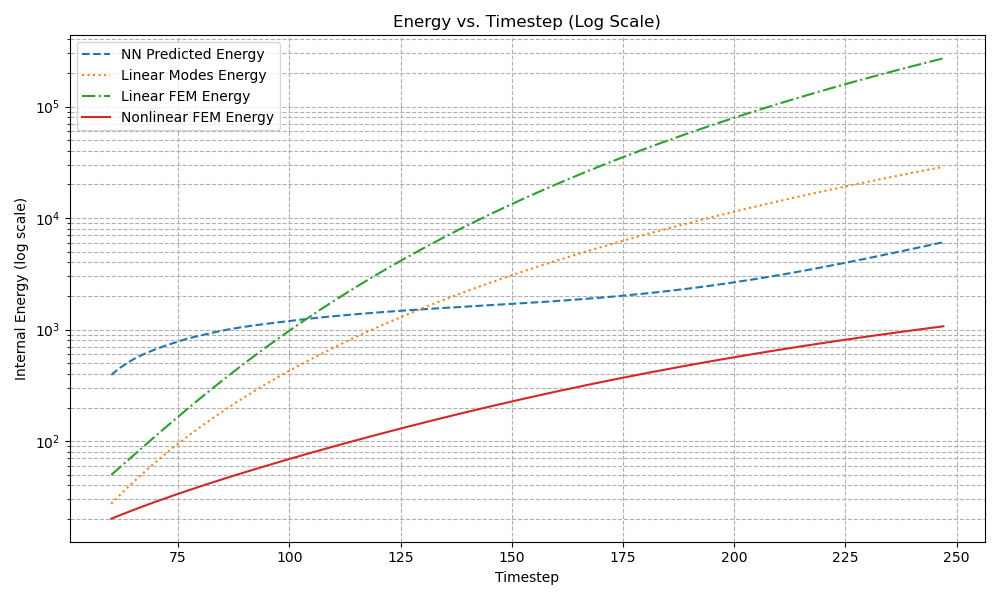
\includegraphics[width=0.8\textwidth]{Images/beam_dynamic_energy.png}
    \caption{Internal mechanical energy of the cantilever beam as a function of time for the dynamic validation. The neural modes model (blue) and the linear modes model (orange) are compared against the ground truth obtained from the nonlinear FEM solution (green). The neural modes model manages to keep the energy at a level that is much closer to the ground truth, while the linear modes model diverges significantly from it.}
    \label{fig:dynamic_validation_energy_comparison}
    \end{figure}




\FloatBarrier % Place this after the section where you want to stop floats from moving forward